\section[Single Particle Detection]{Single Particle Detection}

\begin{frame}{Project Overview}
\begin{itemize}
    \item \textbf{Goal}: Implement and evaluate LodeSTAR for particle detection
    \item \textbf{Scope}: Single-particle detection on synthetic microscopy images
    \item \textbf{Particle Types}: Janus, Ring, Spot, Ellipse, Rod
    \item \textbf{Implementation}: PyTorch + DeepTrack + PyTorch Lightning
    \item \textbf{Tracking}: Logger and Weights \& Biases (WandB) for experiment monitoring
\end{itemize}
\end{frame}

\begin{frame}{Data Generation Pipeline}
\begin{columns}
\begin{column}{0.6\textwidth}
\textbf{Image Generation:}
\begin{itemize}
    \item \textbf{Synthetic particles} with realistic parameters
    \item \textbf{Multiple datasets} for different scenarios:
    \begin{itemize}
        \item Same shape, same size
        \item Same shape, different size
        \item Different shape, same size
        \item Different shape, different size
    \end{itemize}
    \item \textbf{XML annotations} with bounding boxes and SNR values
\end{itemize}
\end{column}
\begin{column}{0.4\textwidth}
\textbf{Technical Details:}
\begin{itemize}
    \item \textbf{Image size}: 416$\times$416 pixels
    \item \textbf{SNR range}: 1-30
    \item \textbf{Intensity range}: 0.1-1.0
    \item \textbf{Particle parameters}: Type-specific values
    \item \textbf{100 images} per dataset type
\end{itemize}
\end{column}
\end{columns}
\end{frame}

\begin{frame}{Sample Images Generation}
\textbf{Sample Images:}
\begin{itemize}
    \item \textbf{Clean samples} for each particle type
    \item \textbf{50$\times$50 pixels} for training
    \item \textbf{Fixed SNR} (10) for consistent performance identical with training datasets
    \item \textbf{Realistic parameters} for each particle type
    \item \textbf{Stored in} \texttt{data/Samples/}
\end{itemize}
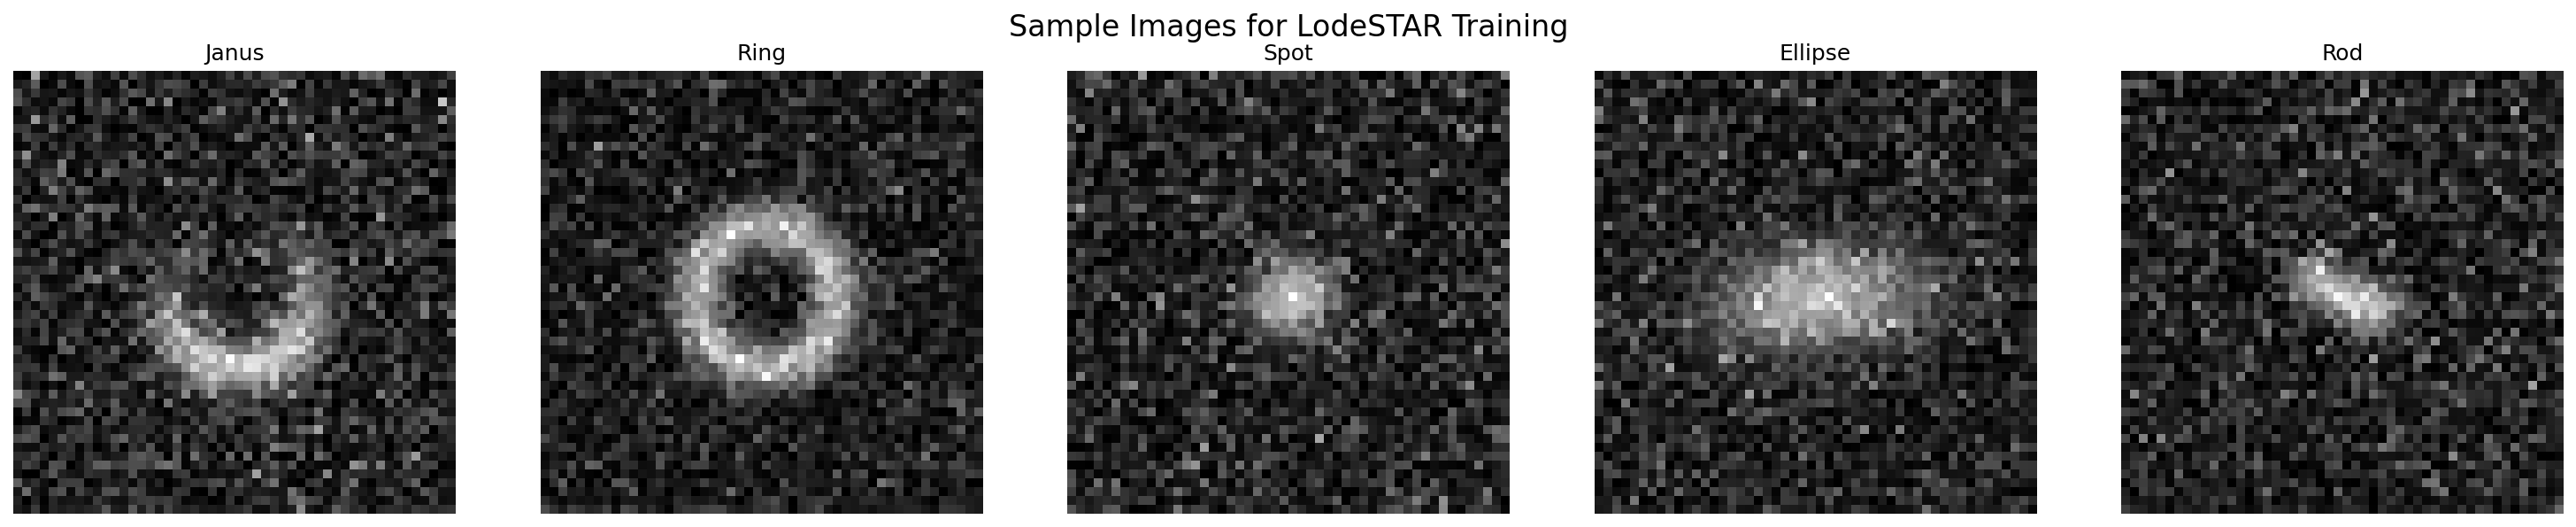
\includegraphics[width=\textwidth]{imglib/sample_overview.png}
\end{frame}

\begin{frame}{Training Pipeline Implementation}
\begin{columns}
\begin{column}{0.6\textwidth}
\textbf{Training Setup:}
\begin{itemize}
    \item \textbf{Single-particle models} for each particle type
    \item \textbf{Data augmentation}: Random intensity augmentation(rotation and translation are implemented implicitly)
    \item \textbf{400 samples per epoch} (configurable)
    \item \textbf{200 epochs} maximum training
    \item \textbf{Batch size}: 8 (balanced for memory)
\end{itemize}
\end{column}
\begin{column}{0.4\textwidth}
\textbf{Technical Stack:}
\begin{itemize}
    \item \textbf{PyTorch Lightning} for training
    \item \textbf{DeepTrack} for data pipelines
    \item \textbf{WandB} for experiment tracking
    \item \textbf{Mixed precision} training (16-bit)
    \item \textbf{GPU acceleration} when available
\end{itemize}
\end{column}
\end{columns}
\end{frame}

\begin{frame}{Training Configuration}
\begin{center}
\begin{tabular}{|c|c|}
\hline
\textbf{Parameter} & \textbf{Value} \\
\hline
Learning Rate & 0.0001 \\
\hline
Batch Size & 8 \\
\hline
Max Epochs & 200 \\
\hline
N Transforms & 4 \\
\hline
\end{tabular}
\end{center}

\end{frame}

\begin{frame}{Detection Scoring Metric}
    \textbf{Detection Score Calculation:}
    \begin{itemize}
        \item The model predicts a weight map ($w$) and local consistency ($b$) is calculated from the predictions.
        \item The final detection score ($S$) combines these metrics using geometric weighting:
        \begin{equation*}
            S = w^\alpha \cdot b^\beta
        \end{equation*}
        \item \textbf{Parameters:}
        \begin{itemize}
            \item $\alpha$: Weight for the predicted weight-map (confidence)
            \item $\beta$: Weight for the local consistency metric
            \item \textbf{Cutoff}: Threshold for valid detections ($S > \text{cutoff}$)
        \end{itemize}
        \item These parameters are tunable for each particle type to optimize performance.
    \end{itemize}
\end{frame}

\begin{frame}{Testing Pipeline \& Results}
\begin{columns}
\begin{column}{0.6\textwidth}
\textbf{Testing Setup:}
\begin{itemize}
    \item \textbf{Load trained models} from checkpoints
    \item \textbf{Test on generated datasets} in \texttt{data/Testing/}
    \item \textbf{Parse XML annotations} for ground truth
    \item \textbf{Calculate detection metrics}: Precision, Recall, F1
    \item \textbf{Distance threshold}: 20 pixels for positive detection
\end{itemize}
\end{column}
\begin{column}{0.4\textwidth}
\textbf{Training Success:}
\begin{itemize}
    \item \textbf{All 5 models} completed 200 epochs
    \item \textbf{Loss convergence} observed
    \item \textbf{Checkpoints saved} every 50 epochs
    \item \textbf{WandB logging} active
    \item \textbf{Model weights} exported
\end{itemize}
\end{column}
\end{columns}
\end{frame}